\begin{quote}
	\textit{``If the chaos of the nineties reflects a radical shift in the paradigms of visual literacy, the final shift away from the Lascaux/Gutenberg tradition of a pre-holographic society, what should we expect from this newer technology, with his promise of discrete encoding and subsequent reconstruction of the full range of sensory perception?''}
\end{quote}
\hfill \textit{Burning Chrome, William Gibson}
\\
\\

%=========================================================================================================

\label{chapter-conclusions}

Alternate realities have fascinated mankind since early prehistory and with the advent of the computer and the smartphone we have seen the rise of many different categories of alternate reality that replace, augment, diminish and mix with our familiar real world to expand our capabilities, our understanding and our entertainment.

This thesis has introduced parallel reality as a new category of alternate reality that comprises two environments, one real and the other virtual, each complete unto itself and wherein the user may freely switch between them. The benefits that such a system imparts upon the user by granting them the ability to explore parallel real and virtual environments in tandem has been shown by developing a parallel reality platform, Mirrorshades, and applying it to a use case within the realm of cultural heritage, with evaluation of these studies leading to a number of best practices for future parallel reality endeavours.

\begin{figure}[h]
	\begin{center}
		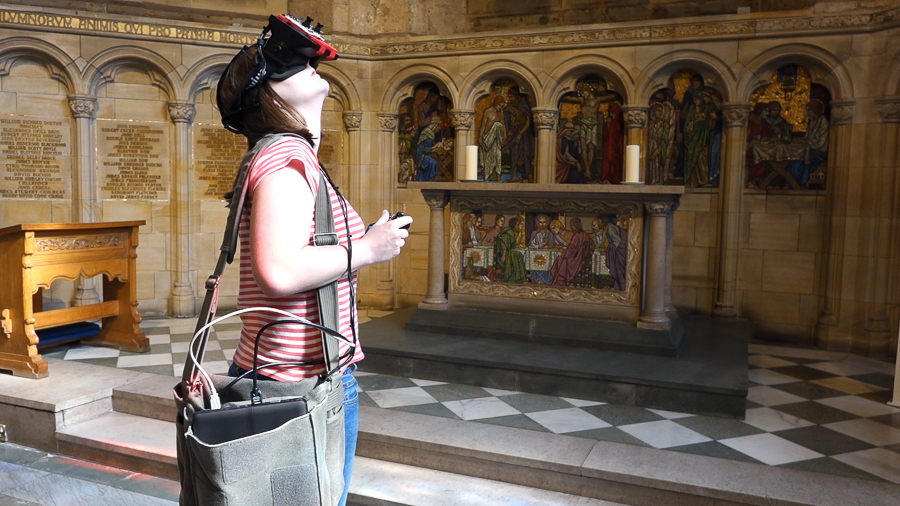
\includegraphics[width=\textwidth]{participant-f-4.jpg}
		\caption{The \textit{Mirrorshades} parallel reality platform in use.}
		\label{participant-f-4.jpg}
	\end{center}	
\end{figure}

%=========================================================================================================

\section{Contributions}

As listed in section \ref{intro-contributions} the contributions of this thesis can be summarized as follows;

\begin{itemize}
	\item The introduction of parallel reality as a new category of alternate reality that allows users to experience two complete environments in tandem and represents an approach for mitigation of the vacancy problem.
	\item The framing of parallel reality through a thorough investigation and extension of previous taxonomies that classify and distinguish alternate reality terminologies.
	\item The creation of the combined Milgram/Waterworth model for visualising alternate reality experiences, including those of parallel reality systems.
	\item Development of a parallel reality platform, dubbed Mirrorshades, that combines new virtual reality hardware with novel indoor positioning technology.
	\item Evaluation of the Mirrorshades platform through user studies of a real world use case study within the realm of cultural heritage, including the application of an established presence questionnaire to parallel reality.
	\item Discussion and creation of a set of best practices for future parallel reality endeavours.
\end{itemize}

%=========================================================================================================

\section{Future Work}

Parallel reality has been presented in this thesis as a new category of alternate reality with the Mirrorshades platform representing the first involved effort at assembling a system within this new categorisation.

%Hardware
Regarding the hardware of the Mirrorshades platform gives rise to an obvious avenue for improvement. Rather than encumbering a user with a bulky, heavy satchel containing a laptop computer, battery pack and myriad wires, and occupying both of their hands with a smartphone and controller, a hardware platform such as Samsung's Gear VR, which unfortunately did not exist in time for inclusion in this thesis, would have a drastic effect upon the comfort of the system and the ability to quickly and easily deploy it in less pre-rehearsed experimental settings.

%Domain/Evaluation
Evaluation of this platform was centred upon an application within the domain of cultural heritage, however parallel reality as a concept can surely be applied to many other areas to great benefit, both serious and not so serious.

%Vacancy/PoSR
PoSR

%=========================================================================================================

\section{Final Thoughts}

Final quote?

%=========================================================================================================